\documentclass{article}

% content/resources/templates/preamble.tex
\usepackage[margin=0.6in]{geometry}
\author{Milav Dabgar}
\usepackage{amsmath,amssymb,amsthm}
\usepackage{booktabs}
\usepackage{multirow}
\usepackage{xcolor}
\usepackage{tcolorbox}
\tcbuselibrary{breakable,skins}
\usepackage[colorlinks=true,linkcolor=blue]{hyperref}
\usepackage{titlesec}
\usepackage{enumitem}
\usepackage{tikz}
\usepackage{pgfplots}
\usepackage{circuitikz}
\usepackage[version=4]{mhchem}
\usepackage{longtable}
\usepackage{array}
\usepackage{float}
\usepackage{caption}
\usepackage{listings}

\lstset{
  basicstyle=\small\ttfamily,
  breaklines=true,
  breakatwhitespace=false,
  postbreak=\mbox{\textcolor{red}{$\hookrightarrow$}\space},
  float=false,
  numbers=left,
  numberstyle=\tiny\color{gray},
  numbersep=10pt,
  xleftmargin=2em,
  keywordstyle=\color{blue},
  commentstyle=\color{green!60!black},
  stringstyle=\color{purple},
  backgroundcolor=\color{gray!5},
  showstringspaces=false,
  tabsize=2,
  captionpos=b,
  keepspaces=true,
  columns=flexible
}

\pgfplotsset{compat=1.18}
\usetikzlibrary{shapes,arrows,positioning,calc,patterns,decorations.pathmorphing,decorations.markings,arrows.meta}

% Color scheme
\definecolor{headcolor}{RGB}{0,102,204}
\definecolor{keycolor}{RGB}{220,20,60}
\definecolor{solutioncolor}{RGB}{34,139,34}
\definecolor{mnemoniccolor}{RGB}{148,0,211}
\definecolor{codecolor}{RGB}{0,0,100}

% Spacing
\setlength{\parskip}{3pt}
\setlist[itemize]{nosep}
\setlist[enumerate]{nosep}

% Title formatting
\titleformat{\section}{\Large\bfseries\color{headcolor}}{\thesection}{1em}{}
\titleformat{\subsection}{\large\bfseries\color{headcolor}}{\thesubsection}{1em}{}

% Pandoc tightlist compatibility
\providecommand{\tightlist}{%
  \setlength{\itemsep}{0pt}\setlength{\parskip}{0pt}}

% Pandoc longtable compatibility
\newcounter{none}
\def\thenone{}


% content/resources/templates/english-boxes.tex

% Custom environments
\newtcolorbox{solutionbox}{
 breakable,
 enhanced,
 colback=solutioncolor!5!white,
 colframe=solutioncolor!75!black,
 fonttitle=\bfseries,
 title=Solution
}

\newtcolorbox{solutionboxnobreak}{
 colback=solutioncolor!5!white,
 colframe=solutioncolor!75!black,
 fonttitle=\bfseries,
 title=Solution
}

\newtcolorbox{keyformula}{
 breakable,
 enhanced,
 colback=keycolor!5!white,
 colframe=keycolor!75!black,
 fonttitle=\bfseries,
 title=Key Formula
}

\newtcolorbox{mnemonicboxenv}{
 breakable,
 enhanced,
 colback=mnemoniccolor!5!white,
 colframe=mnemoniccolor!75!black,
 fonttitle=\bfseries,
 title=Mnemonic
}

\newcommand{\mnemonicbox}[1]{%
  \begin{mnemonicboxenv}
    #1
  \end{mnemonicboxenv}
}


% Custom commands for GTU solutions
% This file defines semantic commands for consistent formatting

% Question command with automatic formatting
\newcommand{\question}[2]{%
  \section*{Question #1}%
  \textbf{#2}%
}

% OR question variant
\newcommand{\questionor}[2]{%
  \section*{Question #1 OR}%
  \textbf{#2}%
}

% Proper table environment with caption
\newenvironment{answertable}[1]{%
  \begin{table}[htbp]
  \centering
  \caption{#1}
}{%
  \end{table}
}

% Proper figure environment for diagrams
\newenvironment{answerdiagram}[1]{%
  \begin{figure}[htbp]
  \centering
  \caption{#1}
}{%
  \end{figure}
}

% Semantic markup for key terms
\newcommand{\keyword}[1]{\textbf{#1}}
\newcommand{\code}[1]{\texttt{#1}}
\newcommand{\classname}[1]{\texttt{#1}}
\newcommand{\methodname}[1]{\texttt{#1}}

% Proper quotation marks
\newcommand{\mnemonic}[1]{``#1''}


\usetikzlibrary{mindmap,trees,fit}

\title{Introduction to IT Systems (4311602) - Winter 2024 Solution}
\date{January 09, 2025}

\begin{document}
\maketitle

\section*{Question 1}

\questionmarks{1(a)}{Explain NAND logic gate.}{3}
\begin{solutionbox}
    \textbf{NAND gate} is a universal logic gate that produces output 0 only when all inputs are 1. It is effectively an AND gate followed by a NOT gate.

    \begin{center}
        \begin{tikzpicture}[circuit logic US]
            \node[nand gate, inputs={nn}] (N) at (0,0) {};
            \draw (N.input 1) -- ++(-0.5,0) node[left] {$A$};
            \draw (N.input 2) -- ++(-0.5,0) node[left] {$B$};
            \draw (N.output) -- ++(0.5,0) node[right] {$Y = \overline{A \cdot B}$};
        \end{tikzpicture}
    \end{center}

    \textbf{Truth Table:}
    \begin{center}
        \begin{tabulary}{\linewidth}{C C C}
            \toprule
            $A$ & $B$ & $Y = \overline{A \cdot B}$ \\
            \midrule
            0 & 0 & 1 \\
            0 & 1 & 1 \\
            1 & 0 & 1 \\
            1 & 1 & 0 \\
            \bottomrule
        \end{tabulary}
    \end{center}

    \begin{itemize}
        \item \textbf{Universal Gate}: Can implement any logic function (AND, OR, NOT).
        \item \textbf{Low Power}: Requires fewer transistors in CMOS IC design.
    \end{itemize}
    \begin{mnemonicbox}NOT AND = NAND\end{mnemonicbox}
\end{solutionbox}

\questionmarks{1(b)}{Draw AND logic Gate using NOR Gate only.}{4}
\begin{solutionbox}
    AND gate can be implemented using NOR gates by applying De Morgan's theorem: $A \cdot B = \overline{\overline{A} + \overline{B}}$.
    
    \textbf{Implementation Steps:}
    \begin{enumerate}
        \item Create NOT A using NOR gate ($A$ NOR $A = \overline{A}$).
        \item Create NOT B using NOR gate ($B$ NOR $B = \overline{B}$).
        \item Feed $\overline{A}$ and $\overline{B}$ into a third NOR gate to get $\overline{\overline{A} + \overline{B}} = A \cdot B$.
    \end{enumerate}

    \textbf{Circuit Diagram:}
    \begin{center}
        \begin{tikzpicture}[circuit logic US, scale=1.2]
            % NOT A
            \node[nor gate, inputs={nn}] (N1) at (0,1) {};
            \draw (N1.input 1) -- ++(-0.5,0) coordinate (A);
            \draw (N1.input 2) -- ++(-0.5,0) coordinate (A_copy);
            \draw (A) -- ++(-0.5,0) node[left] {$A$};
            \draw (A) -- (A_copy); % Tie inputs
            
            % NOT B
            \node[nor gate, inputs={nn}] (N2) at (0,-1) {};
            \draw (N2.input 1) -- ++(-0.5,0) coordinate (B);
            \draw (N2.input 2) -- ++(-0.5,0) coordinate (B_copy);
            \draw (B) -- ++(-0.5,0) node[left] {$B$};
            \draw (B) -- (B_copy); % Tie inputs

            % Final NOR
            \node[nor gate, inputs={nn}] (N3) at (2.5,0) {};
            
            \draw (N1.output) -- ++(0.5,0) |- (N3.input 1) node[midway, above] {$\overline{A}$};
            \draw (N2.output) -- ++(0.5,0) |- (N3.input 2) node[midway, below] {$\overline{B}$};
            
            \draw (N3.output) -- ++(0.5,0) node[right] {$Y = A \cdot B$};
        \end{tikzpicture}
    \end{center}
    \begin{mnemonicbox}Double inversion gives original function\end{mnemonicbox}
\end{solutionbox}

\questionmarks{1(c)}{Explain components of Information System with diagram.}{7}
\begin{solutionbox}
    Information System consists of five key components working together to process data into useful information.

    \textbf{System Diagram:}
    \begin{center}
        \begin{tikzpicture}[node distance=2.5cm, auto]
            \node [gtu block] (proc) {Procedures};
            \node [gtu block, above of=proc] (sw) {Software};
            \node [gtu block, below of=proc] (data) {Data};
            \node [gtu block, left of=proc, xshift=-1cm] (hw) {Hardware};
            \node [gtu block, right of=proc, xshift=1cm] (ppl) {People};
            
            \node [left of=hw] (input) {Input};
            \node [right of=ppl] (output) {Output};

            % Arrows
            \draw [gtu arrow] (input) -- (hw);
            \draw [gtu arrow] (hw) -- (proc);
            \draw [gtu arrow] (sw) -- (proc);
            \draw [gtu arrow] (data) -- (proc);
            \draw [gtu arrow] (ppl) -- (proc);
            \draw [gtu arrow] (proc) -- (ppl); 
            \draw [gtu arrow] (ppl) -- (output);
            
            % Enclosing box
            \node [draw=black!50, dashed, fit=(hw) (sw) (data) (ppl) (proc), inner sep=0.5cm, label=above:Information System] {};
        \end{tikzpicture}
    \end{center}

    \textbf{Components:}
    \begin{center}
        \begin{tabulary}{\linewidth}{L L L}
            \toprule
            \textbf{Component} & \textbf{Description} & \textbf{Examples} \\
            \midrule
            \textbf{Hardware} & Physical devices & CPU, Memory, Keyboards \\
            \textbf{Software} & Programs and applications & OS, Applications, Utilities \\
            \textbf{Data} & Raw facts and figures & Numbers, Text, Images \\
            \textbf{Procedures} & Rules and instructions & User manuals, SOPs \\
            \textbf{People} & Users and operators & End users, IT staff \\
            \bottomrule
        \end{tabulary}
    \end{center}
    \begin{mnemonicbox}Hardware Supports Data Processing People\end{mnemonicbox}
\end{solutionbox}

\questionmarks{1(c) OR}{Explain the working of Google Search Engine with example.}{7}
\begin{solutionbox}
    Google Search Engine uses complex algorithms to find and rank web pages based on user queries.

    \textbf{Working Process:}
    \begin{center}
        \begin{tikzpicture}[node distance=2cm, auto]
            \node [gtu block] (crawl) {Crawling\\(Googlebot)};
            \node [gtu block, right of=crawl, node distance=3.5cm] (index) {Indexing\\(Database)};
            \node [gtu block, right of=index, node distance=3.5cm] (rank) {Ranking\\(PageRank)};
            \node [gtu block, right of=rank, node distance=3.5cm] (serve) {Serving\\(Display)};

            \draw [gtu arrow] (crawl) -- (index);
            \draw [gtu arrow] (index) -- (rank);
            \draw [gtu arrow] (rank) -- (serve);
            
            \node [below of=crawl, text width=2.5cm, align=center, font=\footnotesize] {Discover pages};
            \node [below of=index, text width=2.5cm, align=center, font=\footnotesize] {Store content};
            \node [below of=rank, text width=2.5cm, align=center, font=\footnotesize] {Order by relevance};
            \node [below of=serve, text width=2.5cm, align=center, font=\footnotesize] {User results};
        \end{tikzpicture}
    \end{center}

    \textbf{Key Components:}
    \begin{itemize}
        \item \textbf{Crawling}: Spiders/bots browse the web to discover new and updated pages.
        \item \textbf{Indexing}: Analyzing text, images, and video files on pages and storing them in the large database.
        \item \textbf{Ranking}: Using algorithms (like PageRank) to determine the highest quality answers.
        \item \textbf{Serving}: Returning relevant results to the user's query.
    \end{itemize}

    \textbf{Example Search:}
    \begin{itemize}
        \item \textbf{Query}: "Introduction to IT Systems"
        \item \textbf{Process}: Google checks index for "Introduction", "IT", "Systems".
        \item \textbf{Result}: Educational sites (GTU, TutorialsPoint) ranked higher due to relevance and authority.
    \end{itemize}
    \begin{mnemonicbox}Crawl Index Rank Serve\end{mnemonicbox}
\end{solutionbox}

\section*{Question 2}

\questionmarks{2(a)}{Convert $(16.75)_{10} = (\quad)_8$}{3}
\begin{solutionbox}
    Converting decimal $16.75$ to octal requires separate conversion of integer and fractional parts.

    \textbf{1. Integer Part (16):} Divide by 8
    \begin{center}
        \begin{tabular}{c|c|c}
            Division & Quotient & Remainder \\
            \hline
            $16 \div 8$ & 2 & 0 \\
            $2 \div 8$ & 0 & 2 \\
        \end{tabular}
    \end{center}
    Read remainder from bottom to top: $(20)_8$

    \textbf{2. Fractional Part (0.75):} Multiply by 8
    \[ 0.75 \times 8 = 6.00 \rightarrow \text{Integer } 6 \]
    Read integer from top to bottom: $(.6)_8$

    \textbf{Final Answer:}
    \[ (16.75)_{10} = (20.6)_8 \]
    \begin{mnemonicbox}Divide integer, Multiply fraction\end{mnemonicbox}
\end{solutionbox}

\questionmarks{2(b)}{Explain Multiprocessing Operating System.}{4}
\begin{solutionbox}
    \textbf{Multiprocessing OS} manages multiple processors (CPUs) working simultaneously to execute processes.

    \textbf{Architecture:}
    \begin{center}
        \begin{tikzpicture}[node distance=1.5cm]
            \node[gtu block] (mem) at (0,0) {Shared Memory};
            \node[gtu block] (cpu1) at (-3, 2) {CPU 1};
            \node[gtu block] (cpu2) at (0, 2) {CPU 2};
            \node[gtu block] (cpu3) at (3, 2) {CPU 3};
            
            \draw[gtu arrow] (cpu1) -- (mem);
            \draw[gtu arrow] (cpu2) -- (mem);
            \draw[gtu arrow] (cpu3) -- (mem);
            
            \node[draw, dashed, fit=(cpu1) (cpu3) (mem), label=above:Symmetric Multiprocessing] {};
        \end{tikzpicture}
    \end{center}

    \textbf{Key Features:}
    \begin{itemize}
        \item \textbf{Parallel Processing}: Multiple tasks run at the same time.
        \item \textbf{Reliability}: If one CPU fails, others can take over (Fault Tolerance).
        \item \textbf{Throughput}: Increased number of processes completed per unit time.
        \item \textbf{Shared Resources}: CPUs share memory, bus, and I/O.
    \end{itemize}
    \begin{mnemonicbox}Multiple Processors Process Parallel\end{mnemonicbox}
\end{solutionbox}

\questionmarks{2(c)}{Define Operating System. List out and Explain the functions of Operating System.}{7}
\begin{solutionbox}
    \textbf{Definition}: An Operating System (OS) is system software that manages computer hardware and software resources and provides common services for computer programs.

    \textbf{Core Functions:}
    \begin{center}
        \begin{tikzpicture}[node distance=2.5cm, auto]
            \node[gtu block, fill=blue!10] (os) {Operating System};
            
            \node[gtu block, above of=os] (proc) {Process Mgmt};
            \node[gtu block, right of=os, xshift=1cm] (mem) {Memory Mgmt};
            \node[gtu block, below of=os] (file) {File Mgmt};
            \node[gtu block, left of=os, xshift=-1cm] (io) {I/O Mgmt};
            \node[gtu block, below right of=os, xshift=1cm] (sec) {Security};
            
            \draw[gtu arrow] (os) -- (proc);
            \draw[gtu arrow] (os) -- (mem);
            \draw[gtu arrow] (os) -- (file);
            \draw[gtu arrow] (os) -- (io);
            \draw[gtu arrow] (os) -- (sec);
        \end{tikzpicture}
    \end{center}

    \textbf{Detailed Functions:}
    \begin{enumerate}
        \item \textbf{Process Management}: Creation, scheduling, and termination of processes. Example: Multitasking.
        \item \textbf{Memory Management}: Allocation and deallocation of RAM to processes. Example: Virtual Memory.
        \item \textbf{File Management}: Organizing data into files and directories. Example: NTFS, EXT4.
        \item \textbf{I/O Management}: Managing communication with devices via drivers. Example: Printer spooling.
        \item \textbf{Security}: protecting system from unauthorized access. Example: User login.
    \end{enumerate}
    \begin{mnemonicbox}Process Memory Files Input-Output Security\end{mnemonicbox}
\end{solutionbox}

\questionmarks{2(a) OR}{Convert $(1111111.11)_2 = (\quad)_{10}$}{3}
\begin{solutionbox}
    Converting binary to decimal using positional weights ($2^n$).

    \textbf{Binary}: \texttt{1111111.11}
    
    \textbf{Calculation:}
    \begin{align*}
        1 \times 2^6 &= 64 \\
        1 \times 2^5 &= 32 \\
        1 \times 2^4 &= 16 \\
        1 \times 2^3 &= 8 \\
        1 \times 2^2 &= 4 \\
        1 \times 2^1 &= 2 \\
        1 \times 2^0 &= 1 \\
        1 \times 2^{-1} &= 0.5 \\
        1 \times 2^{-2} &= 0.25
    \end{align*}
    
    Sum: $64 + 32 + 16 + 8 + 4 + 2 + 1 + 0.5 + 0.25 = 127.75$

    \textbf{Final Answer:}
    \[ (1111111.11)_2 = (127.75)_{10} \]
    \begin{mnemonicbox}Powers of Two add Together\end{mnemonicbox}
\end{solutionbox}

\questionmarks{2(b) OR}{Explain Batch Operating System.}{4}
\begin{solutionbox}
    \textbf{Batch OS} processes jobs in groups (batches) without user interaction during execution. Similar jobs are grouped together for efficiency.

    \textbf{Working Model:}
    \begin{center}
        \begin{tikzpicture}[node distance=2.5cm, auto]
            \node [gtu block] (users) {Users};
            \node [gtu block, right of=users] (op) {Operator};
            \node [gtu block, right of=op] (batch) {Batches};
            \node [gtu block, right of=batch] (im) {Computer};
            
            \draw [gtu arrow] (users) -- node {Jobs} (op);
            \draw [gtu arrow] (op) -- node {Group} (batch);
            \draw [gtu arrow] (batch) -- node {Process} (im);
        \end{tikzpicture}
    \end{center}

    \textbf{Characteristics:}
    \begin{itemize}
        \item \textbf{No Interaction}: User cannot interact with the job once submitted.
        \item \textbf{Job Queue}: Jobs are executed sequentially (FIFO).
        \item \textbf{Efficiency}: Reduces setup time by grouping similar tasks.
    \end{itemize}
    \begin{mnemonicbox}Batch Jobs Queue Automatically\end{mnemonicbox}
\end{solutionbox}

\questionmarks{2(c) OR}{Explain Architecture and modes of Linux System with Diagram.}{7}
\begin{solutionbox}
    Linux follows a monolithic kernel architecture where the kernel manages all system resources.

    \textbf{System Architecture:}
    \begin{center}
        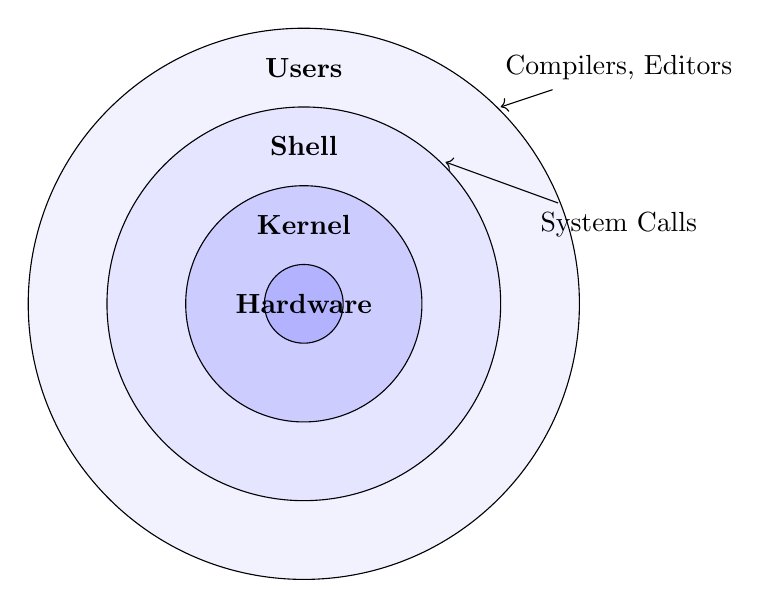
\begin{tikzpicture}
            % Concentric circles
            \draw[fill=blue!5] (0,0) circle (3.5cm);
            \draw[fill=blue!10] (0,0) circle (2.5cm);
            \draw[fill=blue!20] (0,0) circle (1.5cm);
            \draw[fill=blue!30] (0,0) circle (0.5cm);
            
            \node at (0,0) {\textbf{Hardware}};
            \node at (0,1) {\textbf{Kernel}};
            \node at (0,2) {\textbf{Shell}};
            \node at (0,3) {\textbf{Users}};
            
            % Annotations
            \node (apps) at (4,3) {Compilers, Editors};
            \draw[->] (apps) -- (2.5,2.5);
            
            \node (sys) at (4,1) {System Calls};
            \draw[->] (sys) -- (1.8,1.8);
        \end{tikzpicture}
    \end{center}

    \textbf{Operating Modes:}
    \begin{enumerate}
        \item \textbf{User Mode}: Applications run here with restricted access. They cannot access hardware directly.
        \item \textbf{Kernel Mode}: Critical OS code runs here with full access to hardware and memory.
    \end{enumerate}

    \textbf{Key Components:}
    \begin{itemize}
        \item \textbf{Kernel}: Core of the OS, manages CPU, memory, and devices.
        \item \textbf{Shell}: Interface between user and kernel (CLI).
        \item \textbf{Utilities}: Basic programs like \texttt{cp}, \texttt{ls}, etc.
    \end{itemize}
    \begin{mnemonicbox}Users call Kernel for Hardware\end{mnemonicbox}
\end{solutionbox}

\section*{Question 3}

\questionmarks{3(a)}{Differentiate between Open-source Software and Proprietary Software.}{3}
\begin{solutionbox}
    \textbf{Comparison Table:}
    \begin{center}
        \begin{tabulary}{\linewidth}{L L L}
            \toprule
            \textbf{Aspect} & \textbf{Open-source Software} & \textbf{Proprietary Software} \\
            \midrule
            \textbf{Source Code} & Freely available & Closed and protected \\
            \textbf{Cost} & Usually free & Commercial license required \\
            \textbf{Modification} & Can be modified & Cannot be modified \\
            \textbf{Examples} & Linux, Firefox & Windows, MS Office \\
            \textbf{Support} & Community-based & Vendor-provided \\
            \bottomrule
        \end{tabulary}
    \end{center}
    \begin{mnemonicbox}Open Shares, Proprietary Protects\end{mnemonicbox}
\end{solutionbox}

\questionmarks{3(b)}{Explain Ethernet Cable.}{4}
\begin{solutionbox}
    \textbf{Ethernet cable} is the standard wired networking medium for LAN connections.

    \textbf{Cable Types:}
    \begin{center}
        \begin{tikzpicture}[node distance=1.5cm, auto]
            \node [gtu block] (eth) {Ethernet Cables};
            \node [gtu block, below left of=eth, xshift=-2cm] (twisted) {Twisted Pair};
            \node [gtu block, below right of=eth, xshift=2cm] (fiber) {Fiber Optic};
            
            \node [gtu block, below of=twisted] (utp) {UTP (Unshielded)};
            \node [gtu block, below of=utp] (stp) {STP (Shielded)};
            
            \node [gtu block, below of=fiber] (sm) {Single Mode};
            \node [gtu block, below of=sm] (mm) {Multi Mode};
            
            \draw [gtu arrow] (eth) -- (twisted);
            \draw [gtu arrow] (eth) -- (fiber);
            \draw [gtu arrow] (twisted) -- (utp);
            \draw [gtu arrow] (twisted) -- (stp);
            \draw [gtu arrow] (fiber) -- (sm);
            \draw [gtu arrow] (fiber) -- (mm);
        \end{tikzpicture}
    \end{center}

    \textbf{Specifications:}
    \begin{itemize}
        \item \textbf{Cat 5e}: 1 Gbps, 100m.
        \item \textbf{Cat 6}: 10 Gbps, 55m.
        \item \textbf{Connector}: RJ-45 for twisted pair.
    \end{itemize}
    \begin{mnemonicbox}Twisted pairs Carry Digital Data\end{mnemonicbox}
\end{solutionbox}

\questionmarks{3(c)}{Explain Time Division Multiplexing with diagram.}{7}
\begin{solutionbox}
    \textbf{TDM} allows multiple signals to share a single transmission medium by allocating distinct time slots to each signal.

    \textbf{TDM Process:}
    \begin{center}
        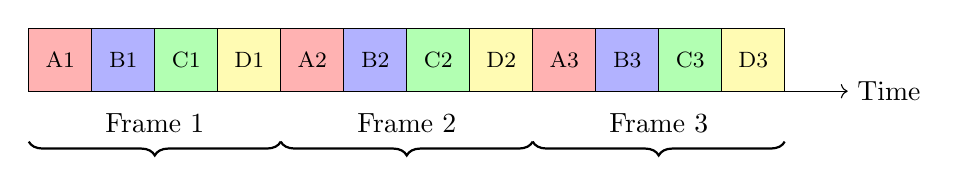
\begin{tikzpicture}[scale=0.8]
            % Axis
            \draw[->] (0,0) -- (13,0) node[right] {Time};
            
            % Slots
            \foreach \x/\c/\col in {0/A1/red!30, 1/B1/blue!30, 2/C1/green!30, 3/D1/yellow!30,
                                    4/A2/red!30, 5/B2/blue!30, 6/C2/green!30, 7/D2/yellow!30,
                                    8/A3/red!30, 9/B3/blue!30, 10/C3/green!30, 11/D3/yellow!30} {
                \draw[fill=\col] (\x,0) rectangle (\x+1,1);
                \node at (\x+0.5, 0.5) {\footnotesize \c};
            }
            
            % Labels
            \node at (2, -0.5) {Frame 1};
            \node at (6, -0.5) {Frame 2};
            \node at (10, -0.5) {Frame 3};
            
            \draw [thick, decoration={brace,mirror,amplitude=5pt},decorate] (0,-0.8) -- (4,-0.8);
            \draw [thick, decoration={brace,mirror,amplitude=5pt},decorate] (4,-0.8) -- (8,-0.8);
            \draw [thick, decoration={brace,mirror,amplitude=5pt},decorate] (8,-0.8) -- (12,-0.8);
        \end{tikzpicture}
    \end{center}

    \textbf{System Components:}
    \begin{enumerate}
        \item \textbf{Multiplexer (MUX)}: Combines input signals into frames.
        \item \textbf{Time Slots}: Fixed duration intervals allocated to channels.
        \item \textbf{Demultiplexer (DEMUX)}: Separates the combined signal at receiver.
    \end{enumerate}
    \begin{mnemonicbox}Time Divides Multiple Signals\end{mnemonicbox}
\end{solutionbox}

\questionmarks{3(a) OR}{Differentiate between Hard Real Time and Soft Real Time Operating System.}{3}
\begin{solutionbox}
    \textbf{Comparison Table:}
    \begin{center}
        \begin{tabulary}{\linewidth}{L L L}
            \toprule
            \textbf{Aspect} & \textbf{Hard Real Time} & \textbf{Soft Real Time} \\
            \midrule
            \textbf{Deadline} & Absolute; must be met & Flexible; preferred \\
            \textbf{Failure Impact} & Catastrophic (System Failure) & degraded performance \\
            \textbf{Examples} & Air Traffic Control, Pacemaker & Video Streaming, Gaming \\
            \textbf{Response} & Guaranteed max time & Best effort \\
            \bottomrule
        \end{tabulary}
    \end{center}
    \begin{mnemonicbox}Hard requires Precision, Soft allows Flexibility\end{mnemonicbox}
\end{solutionbox}

\questionmarks{3(b) OR}{Explain Transmission Modes.}{4}
\begin{solutionbox}
    \textbf{Transmission modes} define the direction of data flow between two devices.

    \begin{center}
        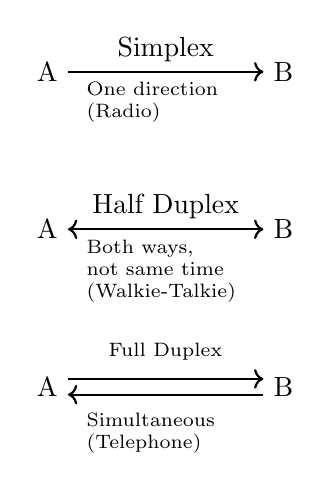
\begin{tikzpicture}[node distance=2cm, auto, thick]
            % Simplex
            \node (s1) at (0,4) {A};
            \node (s2) at (3,4) {B};
            \draw[->] (s1) -- node[above] {Simplex} (s2);
            \node[below, font=\scriptsize, text width=2cm] at (1.5,4) {One direction (Radio)};

            % Half Duplex
            \node (h1) at (0,2) {A};
            \node (h2) at (3,2) {B};
            \draw[<->] (h1) -- node[above] {Half Duplex} (h2);
            \node[below, font=\scriptsize, text width=2cm] at (1.5,2) {Both ways, not same time (Walkie-Talkie)};

            % Full Duplex
            \node (f1) at (0,0) {A};
            \node (f2) at (3,0) {B};
            \draw[transform canvas={yshift=0.1cm}, ->] (f1) -- (f2);
            \draw[transform canvas={yshift=-0.1cm}, <-] (f1) -- (f2);
            \node[above,font=\scriptsize] at (1.5,0.2) {Full Duplex};
            \node[below, font=\scriptsize, text width=2cm] at (1.5,-0.2) {Simultaneous (Telephone)};
        \end{tikzpicture}
    \end{center}

    \textbf{Summary:}
    \begin{itemize}
        \item \textbf{Simplex}: Unidirectional (Keyboard to CPU).
        \item \textbf{Half Duplex}: Bidirectional but one at a time.
        \item \textbf{Full Duplex}: Bidirectional and simultaneous.
    \end{itemize}
    \begin{mnemonicbox}Simplex Single, Half switches, Full flows Both\end{mnemonicbox}
\end{solutionbox}

\questionmarks{3(c) OR}{List out types of Analog Modulation. Explain Amplitude Modulation with diagram.}{7}
\begin{solutionbox}
    \textbf{Types of Analog Modulation:}
    \begin{enumerate}
        \item Amplitude Modulation (AM)
        \item Frequency Modulation (FM)
        \item Phase Modulation (PM)
    \end{enumerate}

    \textbf{Amplitude Modulation (AM)}: The amplitude of the high-frequency carrier wave is varied in accordance with the instantaneous amplitude of the message signal.

    \textbf{Process Diagram:}
    \begin{center}
        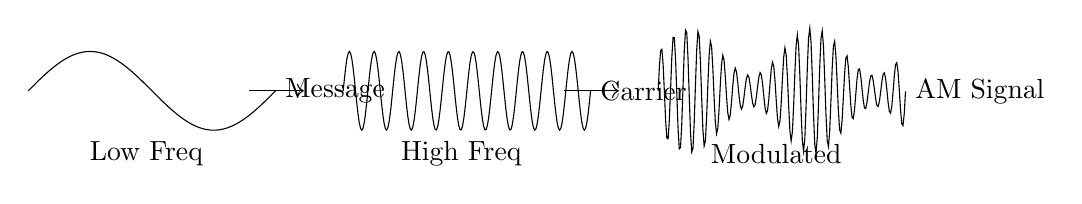
\begin{tikzpicture}
            % Message Signal
            \draw[samples=100, domain=0:2*pi] plot (\x/2, {0.5*sin(\x r)}) node[right] {Message};
            \node at (1.5, -0.8) {Low Freq};

            % Carrier Signal
            \draw[samples=200, domain=0:2*pi, xshift=4cm] plot (\x/2, {0.5*sin(10*\x r)}) node[right] {Carrier};
            \node at (5.5, -0.8) {High Freq};

            % AM Signal (Approximate visual)
            \draw[samples=200, domain=0:4*pi, xshift=8cm, yshift=0] plot (\x/4, {(0.5 + 0.3*sin(\x r)) * sin(10*\x r)}) node[right] {AM Signal};
            \node at (9.5, -0.8) {Modulated};
            
            % Arrows
            \draw[->] (2.8,0) -- (3.5,0);
            \draw[->] (6.8,0) -- (7.5,0);
        \end{tikzpicture}
    \end{center}

    \textbf{Characteristics:}
    \begin{itemize}
        \item \textbf{Modulation Index ($m$)}: Depth of modulation, usually $0 \le m \le 1$.
        \item \textbf{Bandwidth}: $2 \times f_m$ (Twice the message frequency).
        \item \textbf{Equation}: $s(t) = A_c[1 + m\cos(\omega_m t)]\cos(\omega_c t)$.
    \end{itemize}
    \begin{mnemonicbox}Amplitude Varies with Message\end{mnemonicbox}
\end{solutionbox}

\section*{Question 4}

\questionmarks{4(a)}{Draw Diagram of FSK AND PSK.}{3}
\begin{solutionbox}
    \textbf{1. Frequency Shift Keying (FSK):} Frequency changes based on bit (0 or 1).
    \begin{center}
        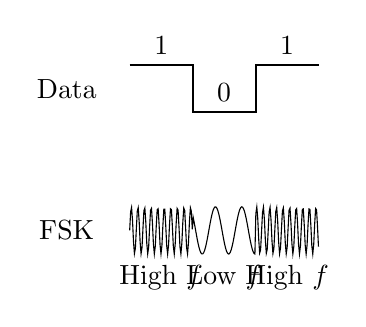
\begin{tikzpicture}[xscale=0.8, yscale=0.6]
            % Bit stream
            \draw[thick] (0,2) -- (1,2) node[midway, above] {1} -- (1,1) -- (2,1) node[midway, above] {0} -- (2,2) -- (3,2) node[midway, above] {1};
            \node at (-1, 1.5) {Data};

            % FSK Signal
            \draw[samples=200, domain=0:3, yshift=-1.5cm] plot (\x, {0.5 * sin ((\x < 1 ? 20 : (\x < 2 ? 5 : 20)) * \x r * 3)}); 
            \node at (-1, -1.5) {FSK};
            \node at (0.5, -2.5) {High $f$}; \node at (1.5, -2.5) {Low $f$}; \node at (2.5, -2.5) {High $f$};
        \end{tikzpicture}
    \end{center}

    \textbf{2. Phase Shift Keying (PSK):} Phase changes by $180^\circ$ on bit transition.
    \begin{center}
        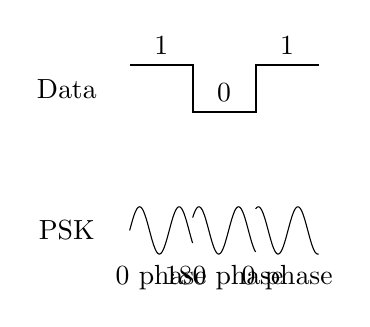
\begin{tikzpicture}[xscale=0.8, yscale=0.6]
            % Bit stream
            \draw[thick] (0,2) -- (1,2) node[midway, above] {1} -- (1,1) -- (2,1) node[midway, above] {0} -- (2,2) -- (3,2) node[midway, above] {1};
            \node at (-1, 1.5) {Data};

            % PSK Signal (visual approx)
            \draw[samples=200, domain=0:1, yshift=-1.5cm] plot (\x, {0.5*sin(10*\x r)});
            \draw[samples=200, domain=1:2, yshift=-1.5cm] plot (\x, {0.5*sin(10*\x r + 3.14159 r)}); % Phase shift
            \draw[samples=200, domain=2:3, yshift=-1.5cm] plot (\x, {0.5*sin(10*\x r)});
            
            \node at (-1, -1.5) {PSK};
            \node at (0.5, -2.5) {0 phase}; \node at (1.5, -2.5) {180 phase}; \node at (2.5, -2.5) {0 phase};
        \end{tikzpicture}
    \end{center}
    \begin{mnemonicbox}FSK changes Frequency, PSK changes Phase\end{mnemonicbox}
\end{solutionbox}

\questionmarks{4(b)}{If number of links in mesh topology are 45 than find maximum number of required nodes.}{4}
\begin{solutionbox}
    \textbf{Formula for Mesh Topology Links:}
    \[ L = \frac{n(n-1)}{2} \]
    Where $n = \text{number of nodes}$.

    \textbf{Given:} $L = 45$.

    \textbf{Calculation:}
    \begin{align*}
        45 &= \frac{n(n-1)}{2} \\
        90 &= n(n-1) \\
        n^2 - n - 90 &= 0
    \end{align*}

    \textbf{Solving Quadratic Equation:} $(n-10)(n+9) = 0$
    
    Since nodes cannot be negative, $n = 10$.

    \textbf{Answer:} Maximum number of nodes is \textbf{10}.
    \begin{mnemonicbox}n nodes need n(n-1)/2 links\end{mnemonicbox}
\end{solutionbox}

\questionmarks{4(c)}{Explain OSI Model with diagram.}{7}
\begin{solutionbox}
    \textbf{OSI (Open Systems Interconnection)} model defines seven layers for network communication.

    \textbf{OSI Layer Stack:}
    \begin{center}
        \begin{tikzpicture}[node distance=0.8cm]
            \node [gtu block, fill=orange!20, text width=5cm] (L7) {Layer 7: Application};
            \node [gtu block, fill=orange!20, text width=5cm, below of=L7] (L6) {Layer 6: Presentation};
            \node [gtu block, fill=orange!20, text width=5cm, below of=L6] (L5) {Layer 5: Session};
            \node [gtu block, fill=green!20, text width=5cm, below of=L5] (L4) {Layer 4: Transport};
            \node [gtu block, fill=green!20, text width=5cm, below of=L4] (L3) {Layer 3: Network};
            \node [gtu block, fill=blue!20, text width=5cm, below of=L3] (L2) {Layer 2: Data Link};
            \node [gtu block, fill=blue!20, text width=5cm, below of=L2] (L1) {Layer 1: Physical};
            
            \draw [->, thick] (L7.east) -- ++(0.5,0) -- ++(0,-5.6) -- (L1.east) node[midway, right] {Data Flow (Encapsulation)};
        \end{tikzpicture}
    \end{center}

    \textbf{Layer Functions:}
    \begin{center}
        \begin{tabulary}{\linewidth}{C L L}
            \toprule
            \textbf{Layer} & \textbf{Function} & \textbf{Protocol/Device} \\
            \midrule
            \textbf{7. Application} & User Interface & HTTP, FTP \\
            \textbf{6. Presentation} & Formatting, Encryption & JPEG, SSL \\
            \textbf{5. Session} & Connection Control & RPC \\
            \textbf{4. Transport} & End-to-end delivery & TCP, UDP \\
            \textbf{3. Network} & Routing (IP Addressing) & Router, IP \\
            \textbf{2. Data Link} & Error detection, MAC & Switch, Ethernet \\
            \textbf{1. Physical} & Bit transmission & Hub, Cable \\
            \bottomrule
        \end{tabulary}
    \end{center}
    \begin{mnemonicbox}All People Seem To Need Data Processing\end{mnemonicbox}
\end{solutionbox}

\questionmarks{4(a) OR}{Explain Classful IPv4 addressing scheme with example.}{3}
\begin{solutionbox}
    \textbf{Classful Addressing:} Divides IP space into 5 classes (A-E).

    \begin{center}
        \begin{tabulary}{\linewidth}{C C C C}
            \toprule
            \textbf{Class} & \textbf{Range} & \textbf{Use} & \textbf{Format} \\
            \midrule
            \textbf{A} & 1 - 126 & Large Networks & N.H.H.H \\
            \textbf{B} & 128 - 191 & Medium & N.N.H.H \\
            \textbf{C} & 192 - 223 & Small (LAN) & N.N.N.H \\
            \textbf{D} & 224 - 239 & Multicast & - \\
            \textbf{E} & 240 - 255 & Research & - \\
            \bottomrule
        \end{tabulary}
    \end{center}

    \textbf{Example:}
    \noindent \textbf{Class C}: \texttt{192.168.1.10}
    \begin{itemize}
        \item Network ID: \texttt{192.168.1}
        \item Host ID: \texttt{10}
        \item Subnet Mask: \texttt{255.255.255.0} (/24)
    \end{itemize}
    \begin{mnemonicbox}A for All, B for Business, C for Company\end{mnemonicbox}
\end{solutionbox}

\questionmarks{4(b) OR}{If number of nodes in mesh topology are 11 than find minimum number of required links.}{4}
\begin{solutionbox}
    \textbf{Formula:} $L = \frac{n(n-1)}{2}$
    
    \textbf{Given:} $n = 11$ nodes.

    \textbf{Calculation:}
    \begin{align*}
        L &= \frac{11(11-1)}{2} \\
          &= \frac{11 \times 10}{2} \\
          &= \frac{110}{2} \\
          &= 55
    \end{align*}

    \textbf{Answer:} 55 links are required.
    \begin{mnemonicbox}Every node connects to Every other\end{mnemonicbox}
\end{solutionbox}

\questionmarks{4(c) OR}{Explain domain name system (DNS) with diagram.}{7}
\begin{solutionbox}
    \textbf{DNS} translates human-readable domain names (example.com) into IP addresses (93.184.216.34) needed for network routing.

    \textbf{DNS Hierarchy:}
    \begin{center}
        \begin{tikzpicture}[level distance=1.5cm, sibling distance=2.5cm, edge from parent/.style={draw,-latex}]
            \node[gtu block] {Root (.)}
                child { node[gtu block] {.com}
                    child { node[gtu block] {google} }
                    child { node[gtu block] {example} }
                }
                child { node[gtu block] {.org} }
                child { node[gtu block] {.edu} };
        \end{tikzpicture}
    \end{center}

    \textbf{Resolution Process Steps:}
    \begin{enumerate}
        \item \textbf{Query}: Client asks "What is IP of google.com?"
        \item \textbf{Local DNS}: Checks cache. If missing, asks Root.
        \item \textbf{Root Server}: Directs to `.com` TLD server.
        \item \textbf{TLD Server}: Directs to `google.com` Authoritative name server.
        \item \textbf{Authoritative}: Returns actual IP address.
    \end{enumerate}

    \textbf{Record Types:}
    \begin{itemize}
        \item \textbf{A}: IPv4 Address.
        \item \textbf{AAAA}: IPv6 Address.
        \item \textbf{MX}: Mail Server.
    \end{itemize}
    \begin{mnemonicbox}Domains Need Systematic name-to-address translation\end{mnemonicbox}
\end{solutionbox}

\section*{Question 5}

\questionmarks{5(a)}{Explain the need of IPv6.}{3}
\begin{solutionbox}
    \textbf{Need for IPv6:} Developed to solve IPv4 address exhaustion.

    \begin{center}
        \begin{tabulary}{\linewidth}{L L L}
            \toprule
            \textbf{Feature} & \textbf{IPv4} & \textbf{IPv6} \\
            \midrule
            \textbf{Address Space} & 4.3 Billion ($2^{32}$) & 340 Undecillion ($2^{128}$) \\
            \textbf{Security} & Optional (IPSec) & Built-in (IPSec) \\
            \textbf{Configuration} & Manual/DHCP & Auto-configuration (SLAAC) \\
            \textbf{Mobility} & Limited & Efficient Mobile IP support \\
            \bottomrule
        \end{tabulary}
    \end{center}
    
    \begin{itemize}
        \item \textbf{IoT Support}: Endless addresses for smart devices.
        \item \textbf{Efficiency}: Simplified header for faster routing.
    \end{itemize}
    \begin{mnemonicbox}IPv6 provides Infinite addresses for Internet growth\end{mnemonicbox}
\end{solutionbox}

\questionmarks{5(b)}{Explain confidentiality using Asymmetric Key encryption.}{4}
\begin{solutionbox}
    \textbf{Asymmetric Encryption} uses a pair of keys: a \textbf{Public Key} for encryption and a \textbf{Private Key} for decryption.

    \textbf{Confidentiality Process:}
    \begin{center}
        \begin{tikzpicture}[node distance=2.5cm, auto]
            \node (sender) {\textbf{Sender}};
            \node [gtu block, right of=sender] (encrypt) {Encrypt};
            \node [gtu block, right of=encrypt] (cipher) {Cipher Text};
            \node [gtu block, right of=cipher] (decrypt) {Decrypt};
            \node [right of=decrypt] (receiver) {\textbf{Receiver}};

            \draw [gtu arrow] (sender) -- node {Msg} (encrypt);
            \draw [gtu arrow] (encrypt) -- (cipher);
            \draw [gtu arrow] (cipher) -- (decrypt);
            \draw [gtu arrow] (decrypt) -- node {Msg} (receiver);

            % Keys
            \node [above of=encrypt, node distance=1.5cm] (pubkey) {Public Key};
            \draw [->, dashed] (pubkey) -- (encrypt);
            
            \node [above of=decrypt, node distance=1.5cm] (privkey) {Private Key};
            \draw [->, dashed] (privkey) -- (decrypt);
            
            \node [below, font=\small, color=gray] at (pubkey) {(Shared)};
            \node [below, font=\small, color=gray] at (privkey) {(Secret)};
        \end{tikzpicture}
    \end{center}

    \textbf{Explanation:}
    \begin{enumerate}
        \item Receiver generates key pair. Shares Public Key.
        \item Sender encrypts message using Receiver's Public Key.
        \item Only Receiver's Private Key can decrypt it.
    \end{enumerate}
    \begin{mnemonicbox}Public locks, Private unlocks\end{mnemonicbox}
\end{solutionbox}

\questionmarks{5(c)}{Explain man-in-middle attack with example.}{7}
\begin{solutionbox}
    \textbf{Man-in-the-Middle (MiTM)}: An attacker intercepts and possibly alters communication between two parties without their knowledge.

    \textbf{Attack Visualization:}
    \begin{center}
        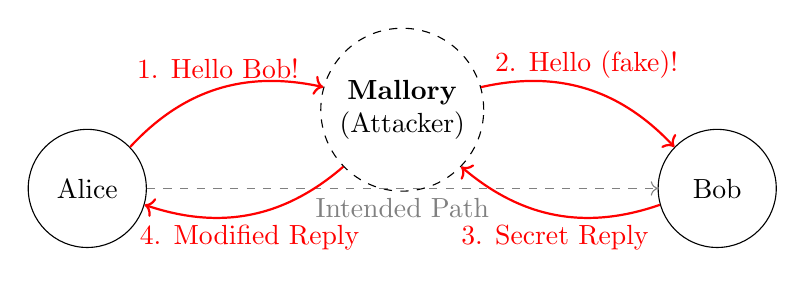
\begin{tikzpicture}[node distance=4cm, auto]
            \node [align=center, draw, circle, minimum size=1.5cm] (alice) {Alice};
            \node [align=center, draw, circle, minimum size=1.5cm, right of=alice, node distance=8cm] (bob)  {Bob};
            \node [align=center, draw, dashed, circle, minimum size=1.5cm, right of=alice, node distance=4cm, yshift=1cm] (mallory) {\textbf{Mallory} \\ (Attacker)};
            
            % Normal path (dashed, intercepted)
            \draw [dashed, ->, color=gray] (alice) -- node[below] {Intended Path} (bob);

            % Attack path
            \draw [->, thick, color=red] (alice) to[bend left] node[above] {1. Hello Bob!} (mallory);
            \draw [->, thick, color=red] (mallory) to[bend left] node[above] {2. Hello (fake)!} (bob);
            
            \draw [->, thick, color=red] (bob) to[bend left] node[below] {3. Secret Reply} (mallory);
            \draw [->, thick, color=red] (mallory) to[bend left] node[below] {4. Modified Reply} (alice);
        \end{tikzpicture}
    \end{center}

    \textbf{Real-world Example (Public WiFi):}
    \begin{enumerate}
        \item \textbf{Scenario}: User connects to fake WiFi "Free\_Airport\_WiFi".
        \item \textbf{Interception}: Attacker sees all unencrypted traffic.
        \item \textbf{Theft}: Passwords and bank details stolen.
    \end{enumerate}
    
    \textbf{Prevention}: Use HTTPS, VPNs, and verify certificates.
    \begin{mnemonicbox}Mallory Intercepts Messages between Alice and Bob\end{mnemonicbox}
\end{solutionbox}

\questionmarks{5(a) OR}{Give the name of OSI model layers with respect to the following devices.\\ 1. Repeater 2. Router 3. Switch}{3}
\begin{solutionbox}
    \textbf{Device Layer Mapping:}
    \begin{center}
        \begin{tabulary}{\linewidth}{C L L}
            \toprule
            \textbf{Device} & \textbf{OSI Layer} & \textbf{Function} \\
            \midrule
            \textbf{Repeater} & Layer 1 (Physical) & Regenerate signal strength \\
            \textbf{Switch} & Layer 2 (Data Link) & Filter/Forward frames by MAC \\
            \textbf{Router} & Layer 3 (Network) & Route packets by IP \\
            \bottomrule
        \end{tabulary}
    \end{center}
    \begin{mnemonicbox}Repeaters work Physically, Switches link Data, Routers route Networks\end{mnemonicbox}
\end{solutionbox}

\questionmarks{5(b) OR}{Explain confidentiality using Symmetric Key encryption.}{4}
\begin{solutionbox}
    \textbf{Symmetric Encryption} uses a \textbf{single shared key} for both encryption and decryption.

    \textbf{Process Flow:}
    \begin{center}
        \begin{tikzpicture}[node distance=2cm, auto]
            \node (pt) {Plain Text};
            \node [gtu block, right of=pt] (enc) {Encryption};
            \node [gtu block, right of=enc] (ct) {Cipher Text};
            \node [gtu block, right of=ct] (dec) {Decryption};
            \node [right of=dec] (pt2) {Plain Text};
            
            \draw [gtu arrow] (pt) -- (enc);
            \draw [gtu arrow] (enc) -- (ct);
            \draw [gtu arrow] (ct) -- (dec);
            \draw [gtu arrow] (dec) -- (pt2);
            
            % Shared Key
            \node [below of=enc, node distance=1.5cm] (key1) {Shared Key};
            \node [below of=dec, node distance=1.5cm] (key2) {Shared Key};
            
            \draw [->, dashed] (key1) -- (enc);
            \draw [->, dashed] (key2) -- (dec);
            \draw [dashed] (key1) -- (key2); % Link keys
        \end{tikzpicture}
    \end{center}

    \textbf{Pros/Cons:}
    \begin{itemize}
        \item \textbf{Speed}: Very fast (AES, DES).
        \item \textbf{Risk}: Key distribution is difficult (if key is stolen, data is lost).
    \end{itemize}
    \begin{mnemonicbox}Same key Encrypts and Decrypts\end{mnemonicbox}
\end{solutionbox}

\questionmarks{5(c) OR}{Explain denial of service attack with example.}{7}
\begin{solutionbox}
    \textbf{DoS (Denial of Service)} attack floods a target with traffic to make it unavailable to legitimate users.

    \textbf{Attack Types Hierarchy:}
    \begin{center}
        \begin{tikzpicture}[level distance=1.5cm, sibling distance=4cm, edge from parent/.style={draw,-latex}]
            \node[gtu block] {DoS Attacks}
                child { node[gtu block] {Volume Based}
                    child { node {UDP Flood} }
                    child { node {ICMP Flood} }
                }
                child { node[gtu block] {Protocol Based}
                    child { node {SYN Flood} }
                    child { node {Ping of Death} }
                }
                child { node[gtu block] {App Layer}
                    child { node {HTTP Flood} }
                    child { node {Slowloris} }
                };
        \end{tikzpicture}
    \end{center}

    \textbf{Attack Categories:}
    \begin{center}
        \begin{tabulary}{\linewidth}{L L L L}
            \toprule
            \textbf{Type} & \textbf{Method} & \textbf{Target} & \textbf{Impact} \\
            \midrule
            \textbf{Volume-based} & Flood with traffic & Bandwidth & Network congestion \\
            \textbf{Protocol-based} & Exploit protocol weakness & Server resources & Service unavailability \\
            \textbf{Application-based} & Target application layer & Application server & Service degradation \\
            \bottomrule
        \end{tabulary}
    \end{center}

    \textbf{Real-world Example - DDoS on E-commerce:}
    \begin{itemize}
        \item \textbf{Target}: Online shopping website during sale season.
        \item \textbf{Method}: Botnet of 10,000 infected computers.
        \item \textbf{Attack}: Each bot sends 100 requests per second.
        \item \textbf{Result}: 1 million requests/second overwhelm servers.
        \item \textbf{Impact}: Website crashes, customers cannot purchase, revenue loss.
    \end{itemize}

    \textbf{Common DoS Techniques:}
    \begin{itemize}
        \item \textbf{SYN Flood}: Exploits TCP handshake process.
        \item \textbf{UDP Flood}: Sends large number of UDP packets.
        \item \textbf{Ping of Death}: Oversized ping packets crash systems.
        \item \textbf{Slowloris}: Keeps connections open to exhaust server.
    \end{itemize}

    \textbf{Defense Strategies:}
    \begin{itemize}
        \item \textbf{Rate Limiting}: Restrict requests per IP address.
        \item \textbf{Firewall Rules}: Block suspicious traffic patterns.
        \item \textbf{DDoS Protection}: Use services like CloudFlare or AWS Shield.
        \item \textbf{Load Balancing}: Distribute traffic across multiple servers.
    \end{itemize}

    \textbf{Business Impact:}
    \begin{itemize}
        \item \textbf{Revenue Loss}: Customers cannot access services.
        \item \textbf{Reputation Damage}: Users lose trust in reliability.
        \item \textbf{Operational Cost}: Resources spent on mitigation.
    \end{itemize}
    \begin{mnemonicbox}Deny service by Overwhelming with requests\end{mnemonicbox}
\end{solutionbox}

\end{document}

